% Options for packages loaded elsewhere
\PassOptionsToPackage{unicode}{hyperref}
\PassOptionsToPackage{hyphens}{url}
%
\documentclass[
]{article}
\usepackage{lmodern}
\usepackage{amssymb,amsmath}
\usepackage{ifxetex,ifluatex}
\ifnum 0\ifxetex 1\fi\ifluatex 1\fi=0 % if pdftex
  \usepackage[T1]{fontenc}
  \usepackage[utf8]{inputenc}
  \usepackage{textcomp} % provide euro and other symbols
\else % if luatex or xetex
  \usepackage{unicode-math}
  \defaultfontfeatures{Scale=MatchLowercase}
  \defaultfontfeatures[\rmfamily]{Ligatures=TeX,Scale=1}
\fi
% Use upquote if available, for straight quotes in verbatim environments
\IfFileExists{upquote.sty}{\usepackage{upquote}}{}
\IfFileExists{microtype.sty}{% use microtype if available
  \usepackage[]{microtype}
  \UseMicrotypeSet[protrusion]{basicmath} % disable protrusion for tt fonts
}{}
\makeatletter
\@ifundefined{KOMAClassName}{% if non-KOMA class
  \IfFileExists{parskip.sty}{%
    \usepackage{parskip}
  }{% else
    \setlength{\parindent}{0pt}
    \setlength{\parskip}{6pt plus 2pt minus 1pt}}
}{% if KOMA class
  \KOMAoptions{parskip=half}}
\makeatother
\usepackage{xcolor}
\IfFileExists{xurl.sty}{\usepackage{xurl}}{} % add URL line breaks if available
\IfFileExists{bookmark.sty}{\usepackage{bookmark}}{\usepackage{hyperref}}
\hypersetup{
  pdftitle={Final Report - Kallikrein genes},
  hidelinks,
  pdfcreator={LaTeX via pandoc}}
\urlstyle{same} % disable monospaced font for URLs
\usepackage[margin=1in]{geometry}
\usepackage{color}
\usepackage{fancyvrb}
\newcommand{\VerbBar}{|}
\newcommand{\VERB}{\Verb[commandchars=\\\{\}]}
\DefineVerbatimEnvironment{Highlighting}{Verbatim}{commandchars=\\\{\}}
% Add ',fontsize=\small' for more characters per line
\usepackage{framed}
\definecolor{shadecolor}{RGB}{248,248,248}
\newenvironment{Shaded}{\begin{snugshade}}{\end{snugshade}}
\newcommand{\AlertTok}[1]{\textcolor[rgb]{0.94,0.16,0.16}{#1}}
\newcommand{\AnnotationTok}[1]{\textcolor[rgb]{0.56,0.35,0.01}{\textbf{\textit{#1}}}}
\newcommand{\AttributeTok}[1]{\textcolor[rgb]{0.77,0.63,0.00}{#1}}
\newcommand{\BaseNTok}[1]{\textcolor[rgb]{0.00,0.00,0.81}{#1}}
\newcommand{\BuiltInTok}[1]{#1}
\newcommand{\CharTok}[1]{\textcolor[rgb]{0.31,0.60,0.02}{#1}}
\newcommand{\CommentTok}[1]{\textcolor[rgb]{0.56,0.35,0.01}{\textit{#1}}}
\newcommand{\CommentVarTok}[1]{\textcolor[rgb]{0.56,0.35,0.01}{\textbf{\textit{#1}}}}
\newcommand{\ConstantTok}[1]{\textcolor[rgb]{0.00,0.00,0.00}{#1}}
\newcommand{\ControlFlowTok}[1]{\textcolor[rgb]{0.13,0.29,0.53}{\textbf{#1}}}
\newcommand{\DataTypeTok}[1]{\textcolor[rgb]{0.13,0.29,0.53}{#1}}
\newcommand{\DecValTok}[1]{\textcolor[rgb]{0.00,0.00,0.81}{#1}}
\newcommand{\DocumentationTok}[1]{\textcolor[rgb]{0.56,0.35,0.01}{\textbf{\textit{#1}}}}
\newcommand{\ErrorTok}[1]{\textcolor[rgb]{0.64,0.00,0.00}{\textbf{#1}}}
\newcommand{\ExtensionTok}[1]{#1}
\newcommand{\FloatTok}[1]{\textcolor[rgb]{0.00,0.00,0.81}{#1}}
\newcommand{\FunctionTok}[1]{\textcolor[rgb]{0.00,0.00,0.00}{#1}}
\newcommand{\ImportTok}[1]{#1}
\newcommand{\InformationTok}[1]{\textcolor[rgb]{0.56,0.35,0.01}{\textbf{\textit{#1}}}}
\newcommand{\KeywordTok}[1]{\textcolor[rgb]{0.13,0.29,0.53}{\textbf{#1}}}
\newcommand{\NormalTok}[1]{#1}
\newcommand{\OperatorTok}[1]{\textcolor[rgb]{0.81,0.36,0.00}{\textbf{#1}}}
\newcommand{\OtherTok}[1]{\textcolor[rgb]{0.56,0.35,0.01}{#1}}
\newcommand{\PreprocessorTok}[1]{\textcolor[rgb]{0.56,0.35,0.01}{\textit{#1}}}
\newcommand{\RegionMarkerTok}[1]{#1}
\newcommand{\SpecialCharTok}[1]{\textcolor[rgb]{0.00,0.00,0.00}{#1}}
\newcommand{\SpecialStringTok}[1]{\textcolor[rgb]{0.31,0.60,0.02}{#1}}
\newcommand{\StringTok}[1]{\textcolor[rgb]{0.31,0.60,0.02}{#1}}
\newcommand{\VariableTok}[1]{\textcolor[rgb]{0.00,0.00,0.00}{#1}}
\newcommand{\VerbatimStringTok}[1]{\textcolor[rgb]{0.31,0.60,0.02}{#1}}
\newcommand{\WarningTok}[1]{\textcolor[rgb]{0.56,0.35,0.01}{\textbf{\textit{#1}}}}
\usepackage{graphicx,grffile}
\makeatletter
\def\maxwidth{\ifdim\Gin@nat@width>\linewidth\linewidth\else\Gin@nat@width\fi}
\def\maxheight{\ifdim\Gin@nat@height>\textheight\textheight\else\Gin@nat@height\fi}
\makeatother
% Scale images if necessary, so that they will not overflow the page
% margins by default, and it is still possible to overwrite the defaults
% using explicit options in \includegraphics[width, height, ...]{}
\setkeys{Gin}{width=\maxwidth,height=\maxheight,keepaspectratio}
% Set default figure placement to htbp
\makeatletter
\def\fps@figure{htbp}
\makeatother
\setlength{\emergencystretch}{3em} % prevent overfull lines
\providecommand{\tightlist}{%
  \setlength{\itemsep}{0pt}\setlength{\parskip}{0pt}}
\setcounter{secnumdepth}{-\maxdimen} % remove section numbering

\title{Final Report - Kallikrein genes}
\author{}
\date{\vspace{-2.5em}19.07.2021}

\begin{document}
\maketitle

\thispagestyle{empty}
\hrule
\vspace{0.3cm}
\begin{center}
    \vspace{1cm}
  \large
    \begin{tabular}[c]{l}
     \\

Anouk Dupe, David Eckey, Dustin Schilling, Maria Yemane \\
\\
     \\
    Supervisor:
    Dr. Maria Dinkelacker \\
     \\
    Tutor:
    Nils Mechtel \\
     \\
     \\
    Data Analysis for students of Molecular Biotechnology \\
    \\
    Heidelberg University 
    \vspace{0.3cm} \\
    \end{tabular}
    \end{center}

\begin{center}\rule{0.5\linewidth}{0.5pt}\end{center}

\pagenumbering{gobble}
\pagebreak
\tableofcontents
\pagebreak
\pagenumbering{arabic}

\hypertarget{introduction}{%
\subsection{1. Introduction}\label{introduction}}

KLKs are a family of 15 mammalian secreted serine proteases. Analysis
has shown that the KLK locus is located on chromosome 19 and forms the
largest cluster of contiguous proteases in the entire genome. (Yousef et
al.~2000).\\
All 15 Kallikrein genes are proteolytic enzymes under steroid hormone
regulation and are involved in the regulation of blood pressure, tissue
remodeling, skin desquamation, and many other processes. The structure
of KLK are similar with two beta-drums, two alpha-helices and a distinct
loop involved in the regulation of activity and selectivity. Currently,
the specific role of each Kallikrein is unclear. It is known that they
are involved in the complex regulatory processes, more specifically in
those different signaling cascades.\\
Dysregulation of KLKs are frequently associated with cancer. Their
expression in different tissues and their involvement in different
physiological processes make them potential tumor expression markers
(Fischer and Meyer-Hoffert, 2013).\\
Different expression of Kallikrein genes has been found in many cancer
types.

\hypertarget{quality-control}{%
\subsection{2. Quality control}\label{quality-control}}

To assure the qualtity of the data the steps presented in ``R Course
Micoarray Analysis'' by Dr.~Maria Dinkelacker (2019) were followed. The
main goal of the quality control is to identify and remove microchips,
which show significantly altered gene expression. These differences
would be difficult to remove via variance stabilizing normalisation
(vsn) and could interfere with the rest of the data. Samples that show
odd characteristics will be identified and replaced in the following
quality control. The quality control was performed on the breast cancer
microarray dataset GSE65216 (Maire et al.~2013) and the small cell lung
cancer microarray dataset GSE149507 (Cai et al.~2021).

\hypertarget{quality-control---gse65216-breast-cancer}{%
\subsubsection{2.1 Quality control - GSE65216 breast
cancer}\label{quality-control---gse65216-breast-cancer}}

The examination of the individual arrays showed no alteration which
indicate physical damage. However, for the meansd plot indicated a
slight linear relationship between mean and the varicance. This could
suggest a mean-variance-dependency.

\begin{figure}

{\centering 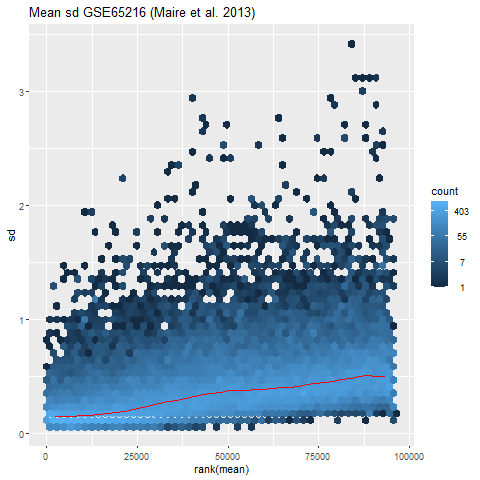
\includegraphics[width=0.5\linewidth]{images/breast_meansdPlot} 

}

\caption{meanSD plot of breast cancer microarray GSE65216.}\label{fig:unnamed-chunk-1}
\end{figure}

In contrast, further quality control did not show any abnormalities.
This the reason why the microchips were not exchangend. The boxplots
showed low fluctuation in gene expression for the 20 arrays after
normalisation. In addition, none of the chips deviate strongly from each
other. In both the density and RNA degradation plot (before and after
normalisation). Also, in scatter plots only linear relationships were
observable. The quality control plots can be viewed in the Github
repository.

\hypertarget{quality-control---gse149507-lung-cancer}{%
\subsubsection{2.2 Quality control - GSE149507 lung
cancer}\label{quality-control---gse149507-lung-cancer}}

One of the chips of the small cell lung cancer microarrays displayed
non-linear relationships in the scatterplots. Since the samples of
dataset GSE149507 for normal and carcinoma tissue are linked to one
patient each. Therefore, the two chips GSM4504109\_SCLC\_05\_ca and
GSM4504110\_SCLC\_05\_n were replaced. The substitute microarrays were
tested again and did not show any discrepancies.

\begin{figure}

{\centering 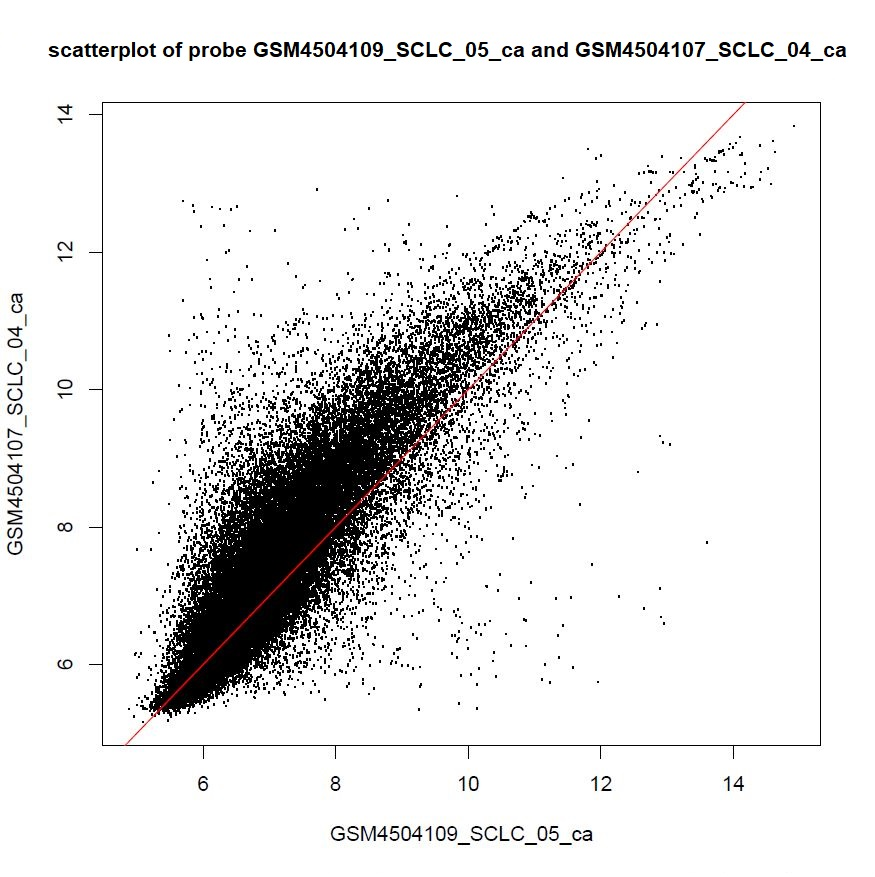
\includegraphics[width=0.5\linewidth]{images/broken_chip_lung} 

}

\caption{Example of scatter plot breast cancer GSE65216.}\label{fig:Broken chip - lung qc}
\end{figure}

\hypertarget{tra-data}{%
\subsection{3. TRA data}\label{tra-data}}

To distinguish between TRA KLK genes and non-TRA KLK genes, a total of 6
TRA datasets were utilized ((Su et al.~2002, 2004), (Roth et al.~2008),
(Lattin et al.~2006), (human GTEX data 2015), (Uhlén et al.~2015)).
These TRA datasets were than unified, which allowed the extraction of
tissue-restricted KLKs according to their transcription number.\\
To get an overview of the distribution of the KLK tissue restriction, a
pie chart was conducted.

Pie charts allow a quick overview of the proportional distribution. The
high prevalence of prostatic kallikrein genes, as well as an occurrence
in esophagus, thyroid and salivary gland is notable. Since six datasets
were combined, annotations that differed for the same tissue type were
fused.

\begin{figure}

{\centering 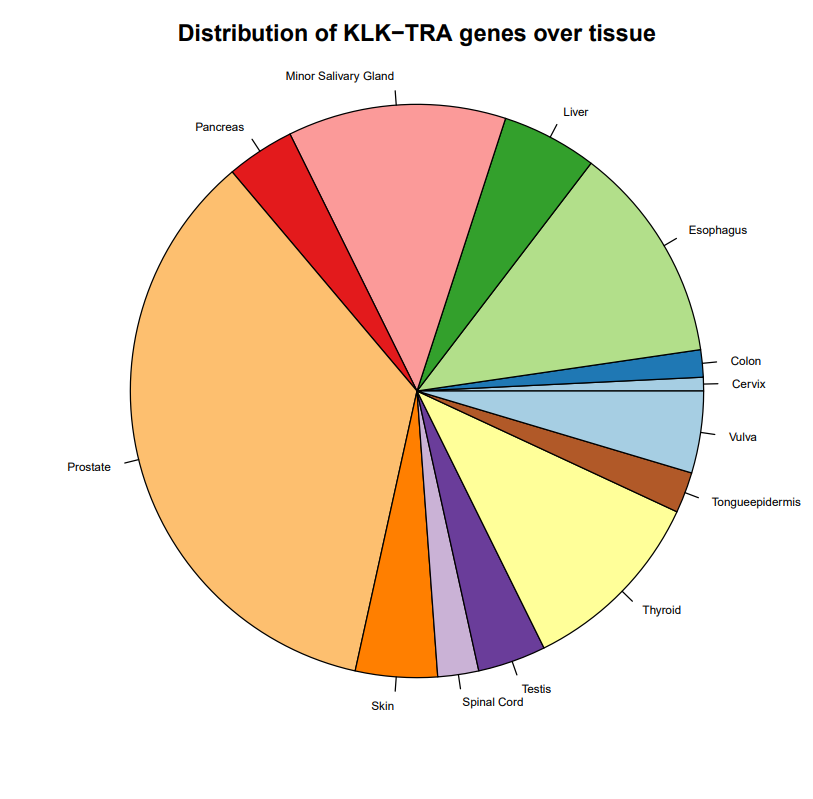
\includegraphics[width=0.5\linewidth]{images/piechart_TRA} 

}

\caption{Tissue specificy of KLK genes - KLK genes from six TRA datasets are combined and sorted for tissue specificity}\label{fig:TRA -piechart}
\end{figure}

\hypertarget{expression-analysis}{%
\subsection{4. Expression Analysis}\label{expression-analysis}}

\hypertarget{breast-cancer-gse65216-maire-et-al.-2013-and-cleanup}{%
\subsection{4.1 Breast cancer GSE65216 (Maire et al.~2013) and
cleanup}\label{breast-cancer-gse65216-maire-et-al.-2013-and-cleanup}}

The breast cancer microarray data GSE65216 (Maire et al.~2013) consists
of 20 samples. Respectively, five samples derive from four mutation
positive tissue: triple negative breast cancer (TNBC), Her2, Luminal A
and Luminal B. Notable, in the microarry data some of the expression
values of KLK isoforms were identical. Therefore, the
Pearson-correlation was determined between all transcripts.Since
isoforms with the correlation of one did not contain additional
information, all of the identical isofroms besindes one were removed. In
the end, 39 identical isoforms are removed, leaving 73 KLK transcripts
for the 15 KLK genes for further analysis. Out of the 73 isoforms, 63
are TRAs, while only 10 are regarded as tissue restricted. Furthermore,
the KLKs are sorted after their names in ascending order for the later
visualization.

\begin{Shaded}
\begin{Highlighting}[]
\CommentTok{# transform dataset - genes on columns}
\NormalTok{df.TRA.KLK.breast <-}\StringTok{ }\KeywordTok{data.frame}\NormalTok{(}\KeywordTok{t}\NormalTok{(TRA.KLK.breast))}

\CommentTok{# Define function for calculating correlation }
\NormalTok{cor.genes <-}\StringTok{ }\ControlFlowTok{function}\NormalTok{(df)\{}
\NormalTok{  df.cor <-}\StringTok{ }\KeywordTok{cor}\NormalTok{(df, }\DataTypeTok{method =} \StringTok{"pearson"}\NormalTok{)}
  \KeywordTok{diag}\NormalTok{(df.cor)=}\OtherTok{NA}
\NormalTok{  df.cor[}\KeywordTok{upper.tri}\NormalTok{(df.cor)]=}\OtherTok{NA}
  \KeywordTok{return}\NormalTok{(}\KeywordTok{data.frame}\NormalTok{(df.cor))}
\NormalTok{\}}

\CommentTok{# amount of identical columns}
\NormalTok{cor.TRA.KLK.breast <-}\StringTok{ }\KeywordTok{cor.genes}\NormalTok{(df.TRA.KLK.breast)}
\KeywordTok{length}\NormalTok{(}\KeywordTok{which}\NormalTok{(cor.TRA.KLK.breast }\OperatorTok{==}\StringTok{ }\DecValTok{1}\NormalTok{))}
\end{Highlighting}
\end{Shaded}

\begin{verbatim}
## [1] 48
\end{verbatim}

\begin{Shaded}
\begin{Highlighting}[]
\CommentTok{# cleanup function }
\NormalTok{genes.cleanup <-}\StringTok{ }\ControlFlowTok{function}\NormalTok{(df)\{}
\NormalTok{  df[}\OperatorTok{!}\KeywordTok{duplicated}\NormalTok{(}\KeywordTok{unclass}\NormalTok{(df))]}
\NormalTok{\}}

\CommentTok{# remove identical columns}
\NormalTok{TRA.KLK.breast.clean <-}\StringTok{ }\KeywordTok{genes.cleanup}\NormalTok{(df.TRA.KLK.breast)}
\KeywordTok{dim}\NormalTok{(TRA.KLK.breast.clean)}
\end{Highlighting}
\end{Shaded}

\begin{verbatim}
## [1] 20 63
\end{verbatim}

\hypertarget{overview-gene-expression}{%
\subsubsection{Overview gene
expression}\label{overview-gene-expression}}

The lowest gene expression value of the first chip is roughly 4, while
the highest gene expression value is around 16. Due to the logarithmic
scale with a base of 2, gene expression doubles every log-fold change of
one.

\begin{Shaded}
\begin{Highlighting}[]
\NormalTok{gene.summary <-}\StringTok{ }\ControlFlowTok{function}\NormalTok{(x)\{}
 \KeywordTok{round}\NormalTok{(}\KeywordTok{apply}\NormalTok{(x, }\DecValTok{2}\NormalTok{, summary), }\DataTypeTok{digits =} \DecValTok{2}\NormalTok{)}
\NormalTok{\}}
\KeywordTok{gene.summary}\NormalTok{(breastExprs)[,}\DecValTok{1}\NormalTok{]}
\end{Highlighting}
\end{Shaded}

\begin{verbatim}
##    Min. 1st Qu.  Median    Mean 3rd Qu.    Max. 
##    4.20    6.28    7.24    7.50    8.43   15.97
\end{verbatim}

The histogram represent the frequency of the present gene expression in
breast cancer samples. It is conspicuous, that the median gene
expression of KLKs is much lower than the overall median gene
expression. This means that most of the KLK gene expression is normally
down-regulated in relation to the whole genome. (Yousef et al.~2004)

\begin{figure}

{\centering 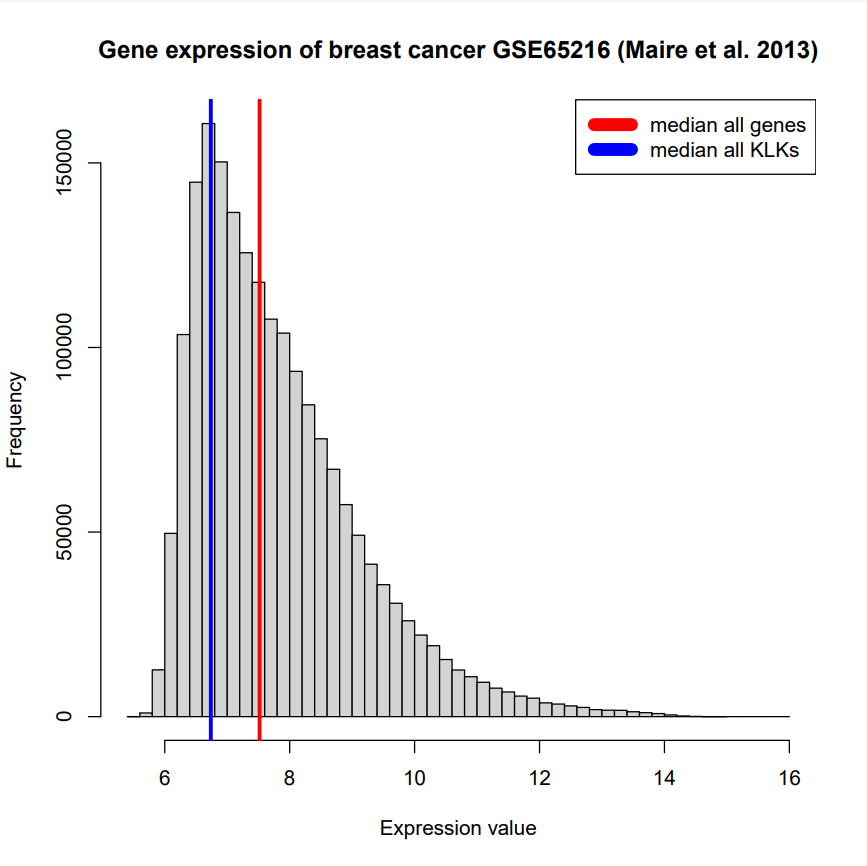
\includegraphics[width=0.5\linewidth]{images/Histogram_breast} 

}

\caption{Histogram of breast cancer gene expression.}\label{fig:Histogram - breast }
\end{figure}

\hypertarget{boxplots}{%
\subsubsection{Boxplots}\label{boxplots}}

The boxplots confirm the fairly low gene expression of KLKs. There are
only two isoforms that exceed the median of the whole genome expression
of the breast cancer set, KLK4.4 and KLK8.8. KLK4 gene expression was
found by Schmitt et al.~to be up-regulated in breast cancer tissue as in
comparison to healthy breast tissue. Thereby, KLK4.4 is part of the
further analysis. In contrast to that, KLK8 seems to be higher expressed
in both normal and cancer tissue (Schmitt et al.~2013).

\begin{figure}

{\centering 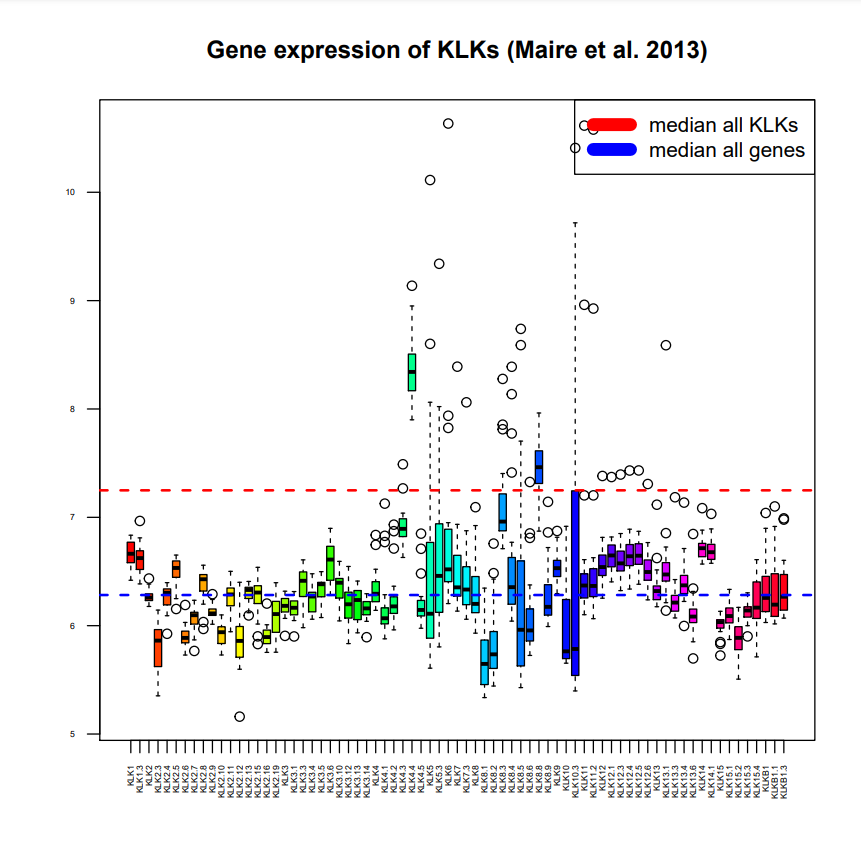
\includegraphics[width=0.5\linewidth]{images/Boxplot_breast} 

}

\caption{Boxplot of KLK gene expression in breast cancer.}\label{fig:Boxplot - breast }
\end{figure}

\hypertarget{heatmap}{%
\subsubsection{Heatmap}\label{heatmap}}

\begin{figure}

{\centering 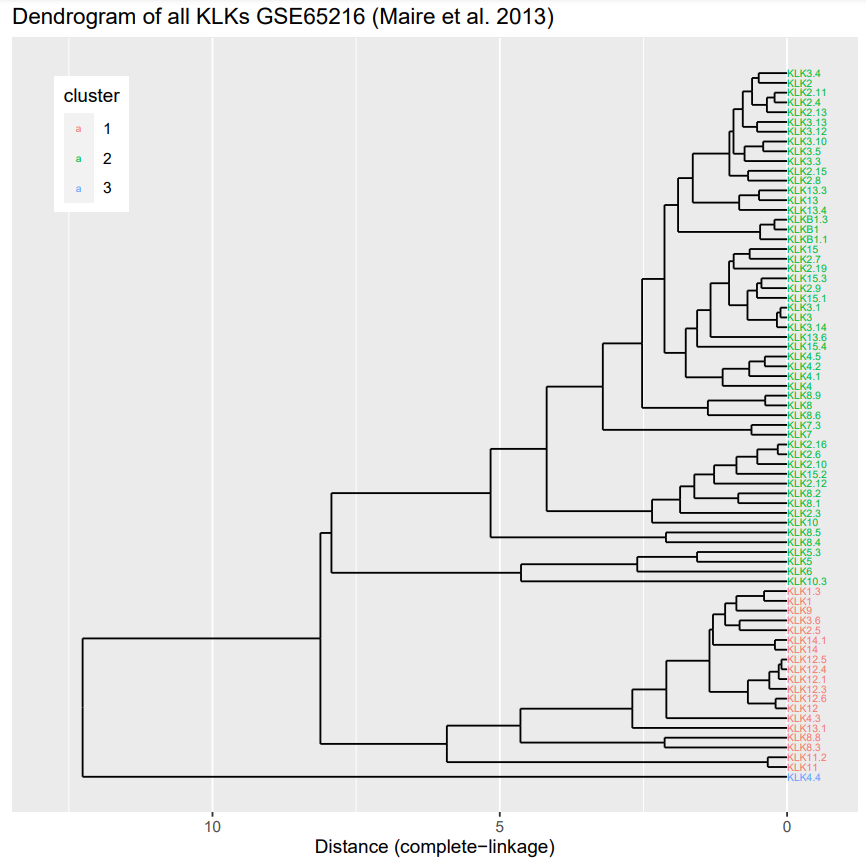
\includegraphics[width=0.5\linewidth]{images/Dendrogram_breast} 

}

\caption{Dendrogram of KLK genes in breast cancer. Clustering is performed after the complete-linkage method. The genes are separated into 3 clusters.}\label{fig:Dendrogram - breast }
\end{figure}

In figure X, KLK4.4 forms its own branch independent of all the others.
As already shown in the boxplots, KLK4.4 was distinctly up-regulated. To
increase the clarity of the heatmap, KLKs are separated into 3 clusters.
Optimal clustering via K-means will still be performed later on. The
dendrogram is the core for the emerging clustering in the heatmap.

\begin{figure}

{\centering 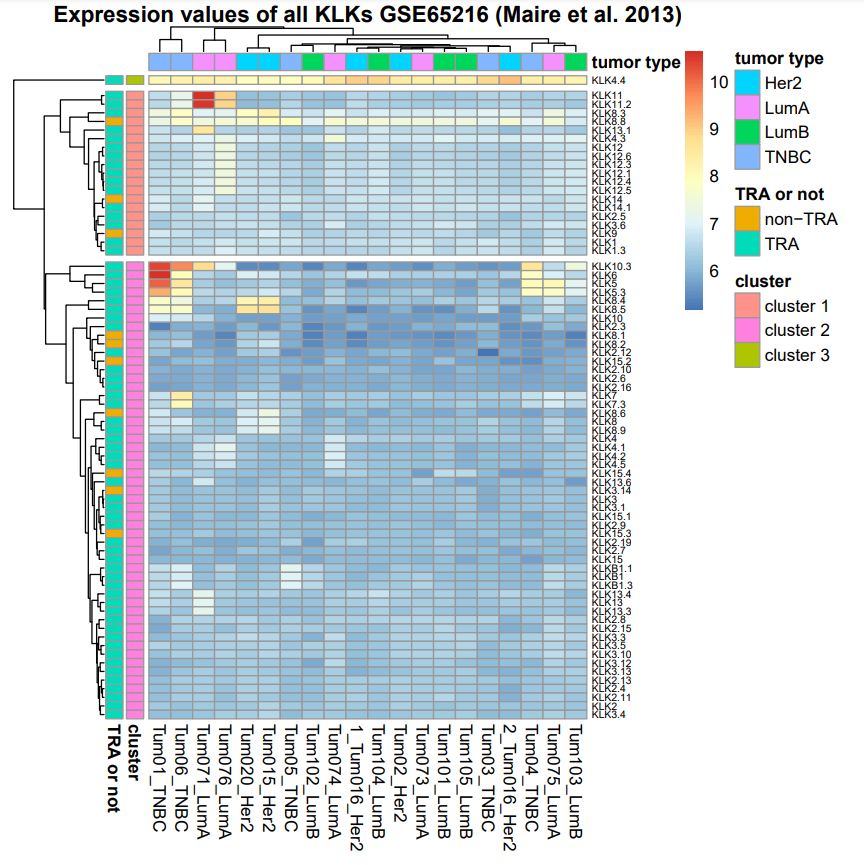
\includegraphics[width=0.5\linewidth]{images/Heatmap_breast} 

}

\caption{Heatmap of KLK gene expression in breast cancer. The samples are annotated corresponding to their mutation type. Additionally, the KLKs are differentiated by their cluster and potential tissue restriction.}\label{fig:Heatmap - breast }
\end{figure}

Once again, KLK4.4 clearly stands out (cluster 3) with an overall
up-regulated gene expression across all samples. In addition, KLK4.4
belongs to the TRA group. Moreover, gene expression in cluster 1 is
higher than within the second cluster. There are only few samples which
seem to have up-regulated KLK transcrips for certain mutation types. For
instance, the tumor sample number 1 and 6 (Tum01\_TNBC and Tum016\_TNBC)
got one of the highest expression values across all the KLKs for
KLK10.3, KLK6 and KLK5. As well as the tumor sample number 71 and 76
(Tum71\_LumA and Tum76\_LumA) for the transcripts KLK11 and KLK11.2.

\hypertarget{principle-component-analysis}{%
\subsubsection{Principle component
analysis}\label{principle-component-analysis}}

The principal component analysis (PCA) reduces multidimensional datasets
into principle components with proportional variance. In this analysis,
PCA was excuted over the samples. Scaling was not included, due to the
data being vsn-normalized. The cumulative variance of the first two
principal components (PCs) yield 72\% of the total variance. Thus, PC1
and PC2 are sufficient for the analysis. The breast cancer samples are
distributed after their respective loadings of KLK gene expression.\\

\begin{figure}

{\centering 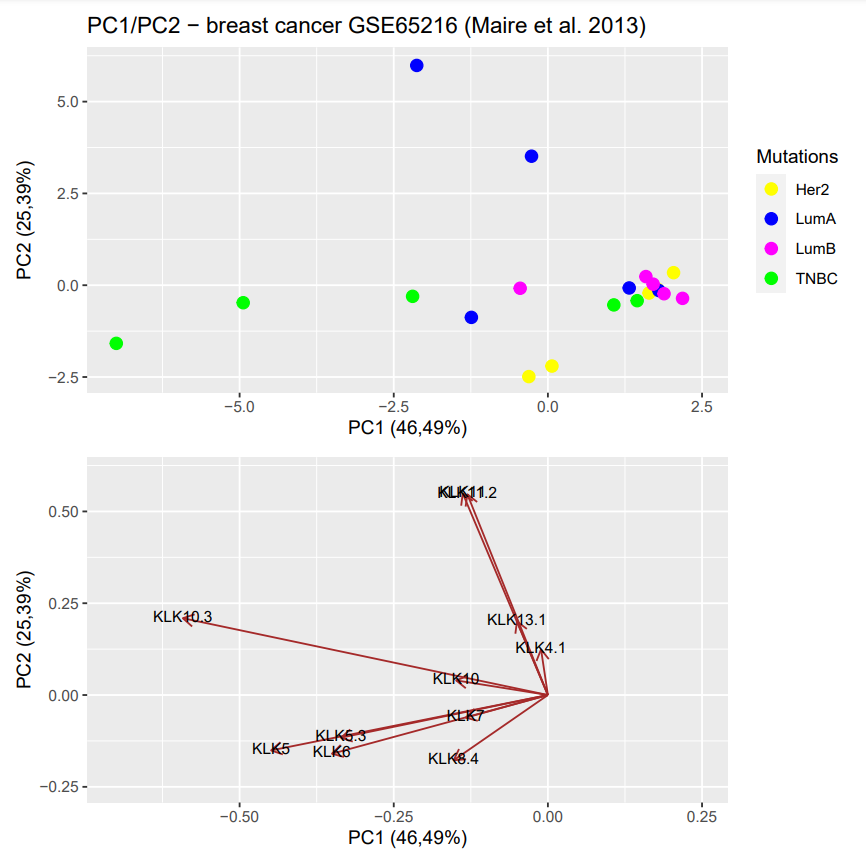
\includegraphics[width=0.5\linewidth]{images/PCAplot_breast} 

}

\caption{PC1 is plotted against PC2. The upper part shows the distribution of the breast cancer samples annotated by their mutation type, while the lower part depicts the 12 highest loadings of the KLK genes. Centering was enabled, scaling was not included.}\label{fig:PCA plot - breast }
\end{figure}

The loadings consists of the the top twelve most differentiated KLK
isoforms. This was conducted by adding absolute values of the rotation
matrix for each individual KLK isoform. Some samples are more
characterized by the expression of KLK11 and KLK11.2. This is mostly the
case for two of the LumA samples. Also, higher expression of KLK11 and
KLK11.2 for the tumor samples 71 and 76 is observable in the heatmap.
Another finding of the PCA is that TNBC mutations are affected by KLK5
and KLK6 expression. Presumably, KLK4.4 is not part of the top twelve
loadings, since it is higher expressed across all tumor samples.

\hypertarget{k-means-clustering}{%
\subsubsection{K-means clustering}\label{k-means-clustering}}

In order to draw conclusions on characteristics and distribution of
different KLKs, k-means was performed. The optimal number of clusters k
was determined with the elbow method. For different cluster counts the
respective within sum of squares (WSS) was computed, a sudden decrease
results in a kink. In this case, the optimal number of clusters is
six.\\
To reduce the dimensions PCA was applied over the KLK genes. In figure X
two of the six clusters are clearly separated. Cluster 1 one contains
KLK4.4 and KLK8.8 and cluster 4 contains KLK5, KLK5.3, KLK6 and KLK10.3.
The respective KLKs out of these two clusters will be further analyzed.
To verify significantly different gene expression in comparison to the
other KLKs hypothesis testing will be used.

\begin{figure}

{\centering 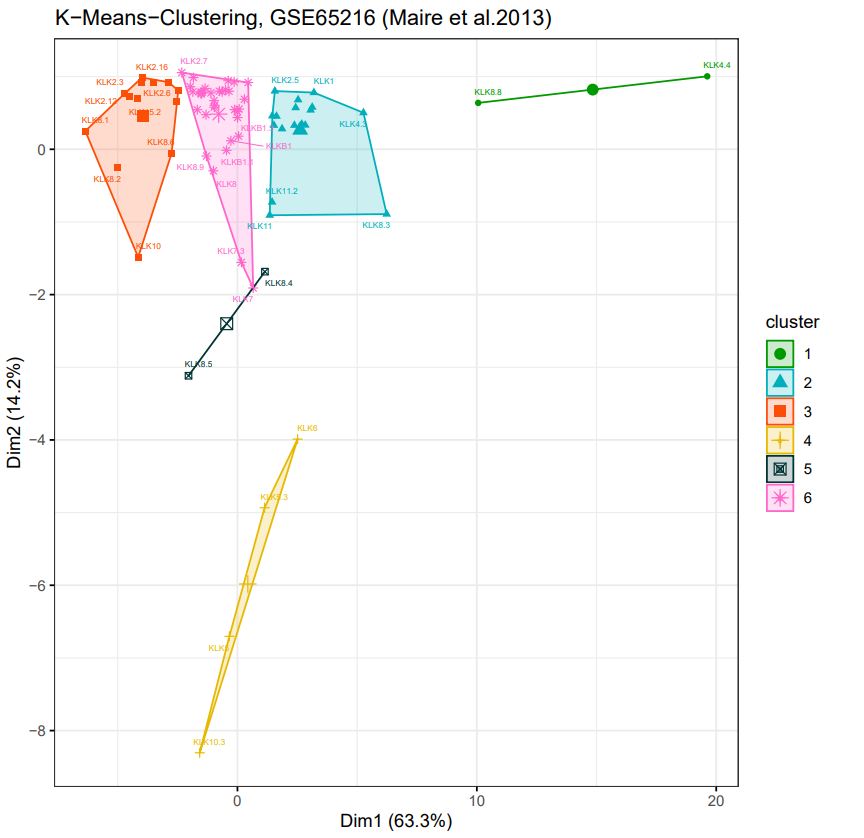
\includegraphics[width=0.5\linewidth]{images/kmeans_6_breast} 

}

\caption{K-means cluster analysis with k = 6 clusters for the breast cancer dataset}\label{fig:K-means plot - breast }
\end{figure}

\hypertarget{hypothesis-testing}{%
\subsubsection{Hypothesis testing}\label{hypothesis-testing}}

The expression values of the KLKs obtained from Marie et al.~were not
normally distributed. Therefore, the non- parametric
Wilcoxon-Mann-Whitney test was applied. The method merges the values of
the two tested samples and ranks the values in an increasing order,
before calculating the p-value. First, the k-means genes of cluster 1
(KLK4.4 and KLK8.8) were tested for over-expression against all other
individual KLKs. Thus, the upper-tail Wilcoxon-test was used. KLK4.4
(TRA) was significantly higher expressed than all other KLKs. Likewise,
KLK8.8 (non-TRA) was significantly higher expressed than all KLK genes,
except KLK4.4. Those results correspond with the observations from the
heatmap and the k-means clustering. Cluster 4 (KLK5, KLK5.3, KLK6,
KLK10.3) was isolated in the k-means clustering. As was mentioned, genes
of this cluster were over-expressed in certain mutation types.
Significant over-expression could not be confirmed, due to the fact that
was no differentiation between the tumor types.

The main characteristic of the dataset from Marie et al.~is the
subdivision into the samples with different mutations (Her2, LumA, LumB,
TNBC). In Figure X, these genes are shown with the subdivision into the
different mutation types. Significant expression differences between
mutation samples are indicated with brackets. A recurring pattern in
Figure X is the significant over-expression of TNBC compared with Her2.
This observation includes KLK5, KLK5.3, KLK10, KLK10.3.

\begin{figure}

{\centering 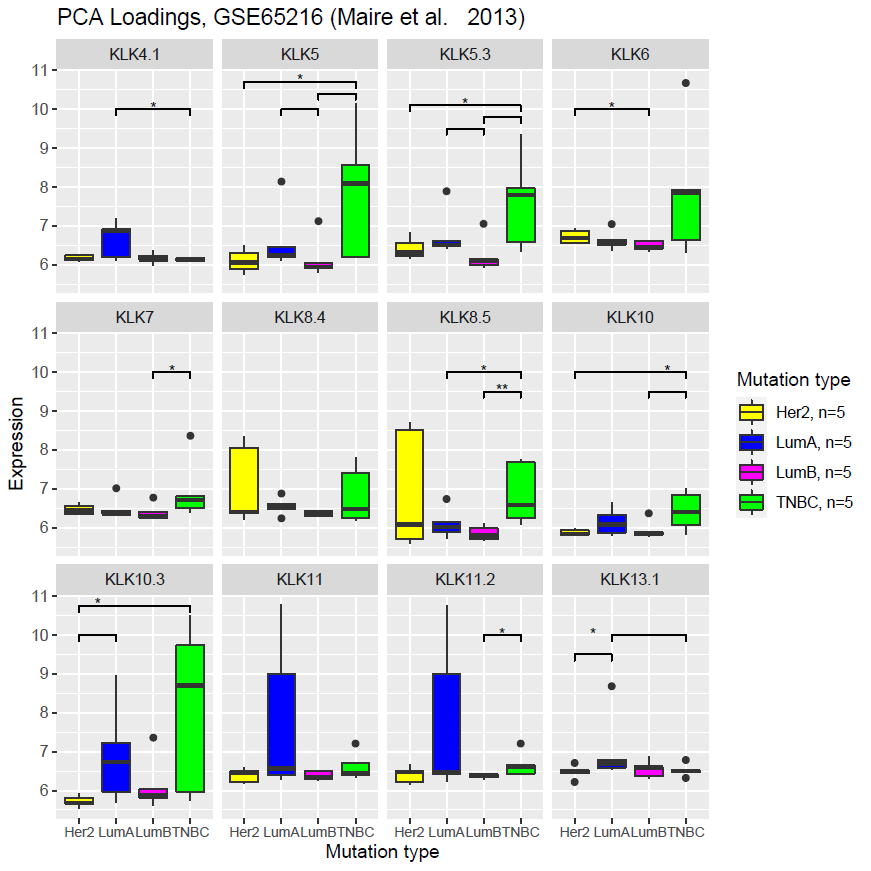
\includegraphics[width=0.5\linewidth]{images/breast_panel_loadings_test} 

}

\caption{Panel plot of the PCA loading genes with significant bars. *: p-value <= 0.5, **: p-value <= 0.01 }\label{fig:Hypothesis test panel plot with significant bars}
\end{figure}

\hypertarget{lung-cancer-gse149507-cai-et-al.-2021}{%
\subsection{4.2 Lung cancer GSE149507 (Cai et
al.~2021)}\label{lung-cancer-gse149507-cai-et-al.-2021}}

The lung cancer microarray GSE149507 (Cai et al.~2021) derives from six
patients with small cell lung cancer. The dataset consists of a total of
twelve samples. Carcinoma tissue and healthy lung tissue, which is
adjacent to the carcinoma, make up six samples each.

\hypertarget{overview-gene-expression-1}{%
\subsubsection{Overview gene
expression}\label{overview-gene-expression-1}}

\begin{figure}

{\centering 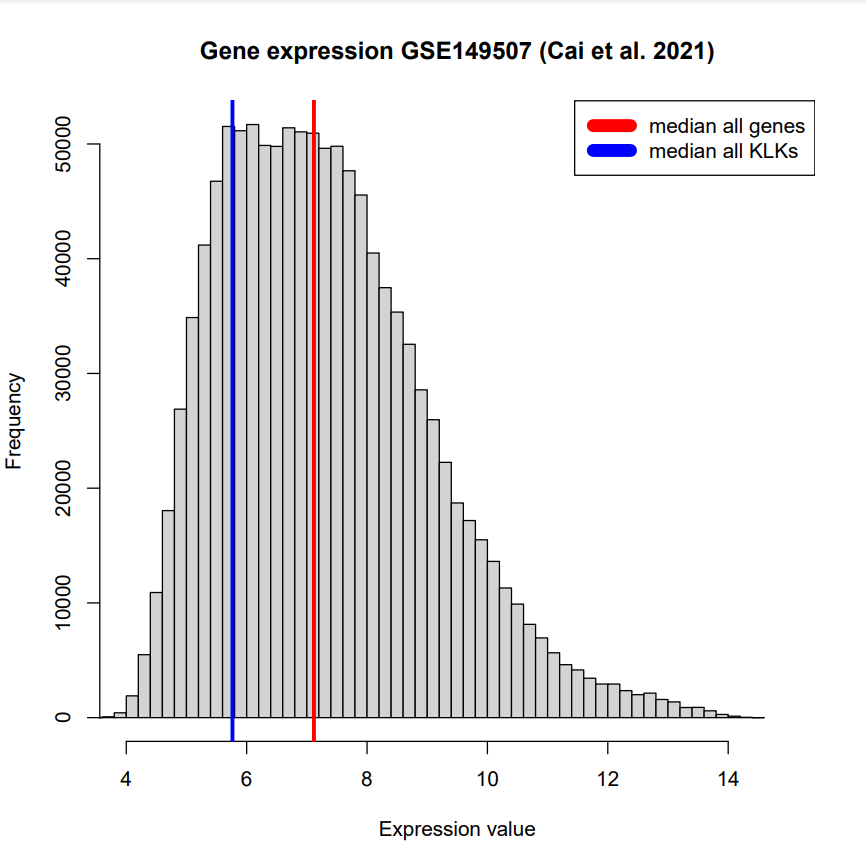
\includegraphics[width=0.5\linewidth]{images/Histogram_lung} 

}

\caption{Histogram of lung cancer gene expression.}\label{fig:Histogram - lung }
\end{figure}

Just as for the breast cancer dataset, the median expression of the KLKs
is beneath the the median of the overall gene expression, since KLKs are
mostly down-regulated (Yousef et al.~2004). However, for the lung cancer
dataset the gene expression values are distributed more evenly, while
the breast cancer histogram represents a right-skewed distribution.

\hypertarget{boxplots-1}{%
\subsubsection{Boxplots}\label{boxplots-1}}

Most of the KLK boxplots are lower than the overall median gene
expression and thereby clearly down-regulated. KLK4.4 clearly stands out
again as the highest expressed KLK gene. In regard to the whole genome
KLK4.4 with an expression value of eight is only slightly above the
overall median gene expression. The boxplot demonstrates that KLK12 and
its isoforms have a high variance and their expression patterns are
similar. A possible reason is that the lung cancer dataset consists of
both normal and healthy tissue, as in comparison to the breast cancer
dataset. In this case, KLK12 and its isofroms a subject for further
investigation to determine whether they are differently expressed
between normal and carcinoma samples.

\begin{figure}

{\centering 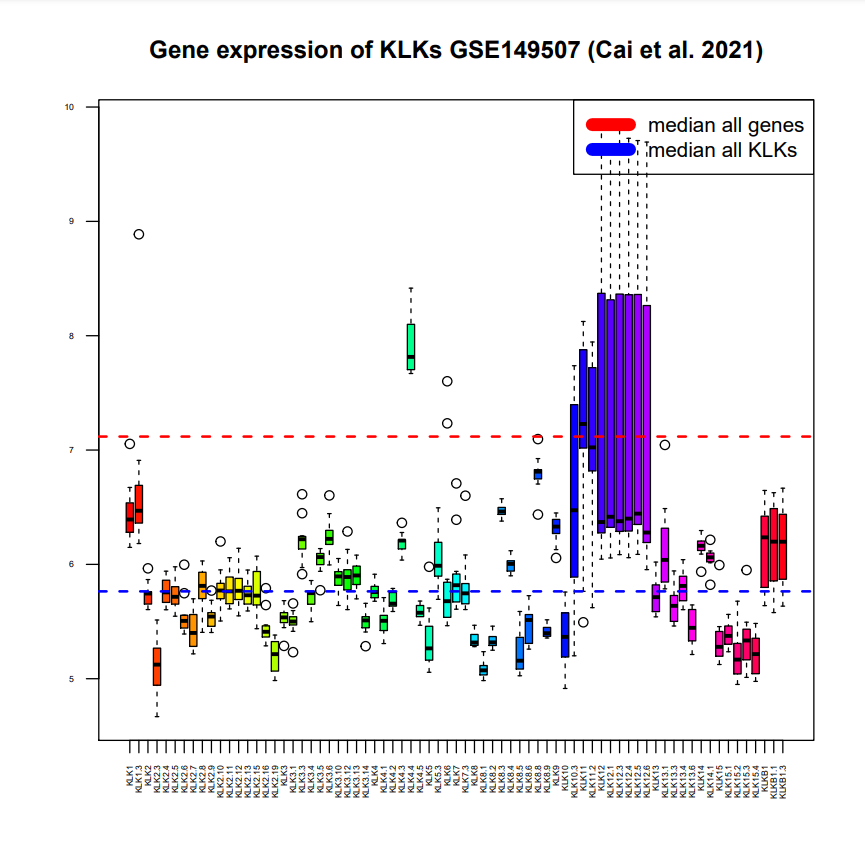
\includegraphics[width=0.5\linewidth]{images/Boxplot_lung} 

}

\caption{Boxplot of KLK gene expression in lung cancer.}\label{fig:Boxplot - lung }
\end{figure}

\hypertarget{heatmap-1}{%
\subsubsection{Heatmap}\label{heatmap-1}}

The lung dataset was split into three clusters with the same method used
for the breast cancer dataset. In addition, the samples are clustered
according to their tissue type being lung carcinoma or healthy tissue.
In the dendrogram of the sample type it is striking that the normal
samples are clustered into one group with additionally two more cancer
samples. Whereas, the other four cancer samples all form their own
distinct group. The clustering of the samples clearly reflects itself in
the KLK11 and KLK12 gene expression. While KLK4.4 is higher expressed
for both normal and carcinoma samples, KLK11 and KLK12 isoforms are
mainly higher expressed for the carcinoma sample. The only exception are
the already mentioned carcinoma samples SCLC\_01 and SCLC\_03.

KLK11 up-regulation in lung cancer was found to have an unfavorable
prognosis for the patient (Borgoño et Diamandis 2004). Four out of the
six cancer samples have slightly up-regulated KLK11 values. The
significance will be tested. The two aforementioned carcinoma samples
SCLC\_01 and SCLC\_03 even got down-regulated KLK11 expression.

\begin{figure}

{\centering 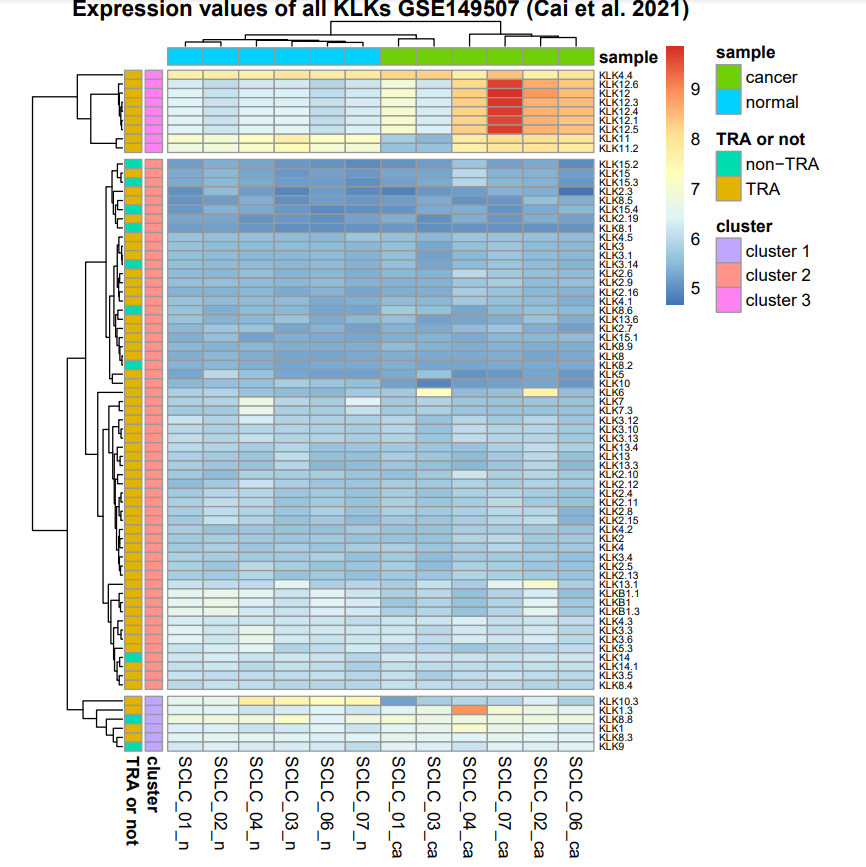
\includegraphics[width=0.5\linewidth]{images/Heatmap_lung} 

}

\caption{Heatmap of KLK gene expression in breast cancer. Carcinoma and normal samples are annotated. Additionally, the KLKs are differentiated by their cluster and potential tissue restriction.}\label{fig:Heatmap - lung }
\end{figure}

\hypertarget{pca}{%
\subsubsection{PCA}\label{pca}}

The first two PCs explain 84\% of the total variance. This high
cumulative variance indicates that the majority of the variance can be
explained by only a few transcripts. As expected, the PCA shows a clear
separation between normal and carcinoma samples. Considering the top
loadings, four of the cancer samples are characterized by KLK12, while
the other two tumor samples SCLC\_01\_ca and SCLC\_03\_ca are mainly
represented by KLK4.4 and KLK6 expression. As in the heatmap, four out
of the six cancer samples have up-regulated KLK12 expression values, the
two cancer samples SCLC\_01\_ca and SCLC\_03\_ca form an exception. They
are rather defined by KLK6 and KLK4.4 expression.

\begin{figure}

{\centering 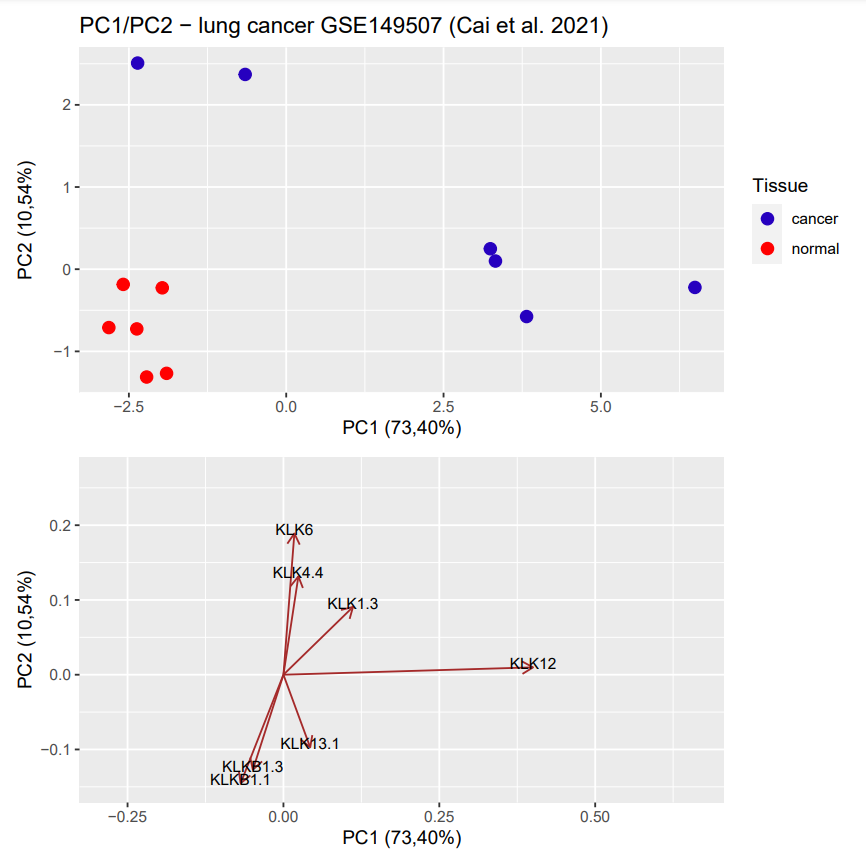
\includegraphics[width=0.5\linewidth]{images/PCAplot_lung} 

}

\caption{PC1 is plotted against PC2. The upper part shows the distribution of the lung cancer samples annotated by their tissue type, while the lower part depicts the top 7 loadings of the KLKs.}\label{fig:PCA plot - lung }
\end{figure}

\hypertarget{clustering---kmeans}{%
\subsubsection{Clustering - kmeans}\label{clustering---kmeans}}

The opimal cluster count was determined with the same method as for the
breast cancer dataset and equaled five. Cluster 5 only consists of KLK12
and its isoforms. KLK4.4 and KLK8.8, which were conspicuous in the
heatmap, are part of cluster 1. The other three clusters containing
genes, which were low expressed in the heatmap, are located next to each
other.

\begin{figure}

{\centering 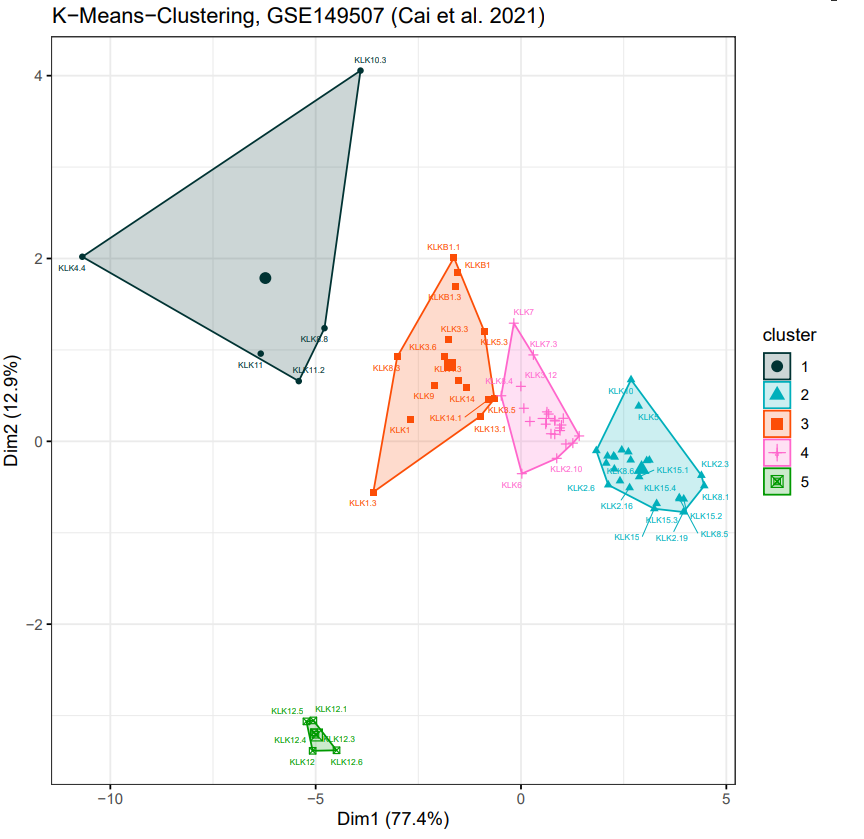
\includegraphics[width=0.5\linewidth]{images/kmeans_5_lung} 

}

\caption{K-means cluster analysis with k = 5 clusters for the lung cancer dataset}\label{fig:K-means plot - lung }
\end{figure}

\hypertarget{hypothesis-testing-1}{%
\subsubsection{Hypothesis testing}\label{hypothesis-testing-1}}

The results of the PCA and the k-means indicate that for some KLKs the
expression differs between the cancerous and normal tissue. Since the
KKLK expression is not normally distributed, the Wilcoxon signed-rank
test was used. In figure X plot A, KLK4.4 was significantly higher
expressed in cancer tissue. Unlike KLK10.3, which was significantly
higher expressed in normal tissue. Plot B shows that KLK12 and its
isoforms are significantly higher expressed in cancer tissue. Also, the
plot visualizes the high similarity within isoforms because only
identical transcripts were removed during the clean up. KLKs that
characterize normal samples in the PCA are shown in plot C. In this
respect, KLKB1.1 and KLKB1.3 are significantly down-regulated in the
cancer tissue. The KLKs which characterized the cancer tissue are shown
in plot D. Here, KLK1.3, KLK4.4, and KLK12 were significantly higher
expressed in cancerous tissue. In summary, five out of seven loadings
were found to have a significant expression difference between the
tissue types. Those results confirm the clear separation of cancer and
normal tissue microchips in the PCA based on KLK expression.\\
In conclusion, the hypothesis tests confirm the clear separation of
cancer and normal tissue sample in the PCA based on KLK expression.

\begin{figure}

{\centering 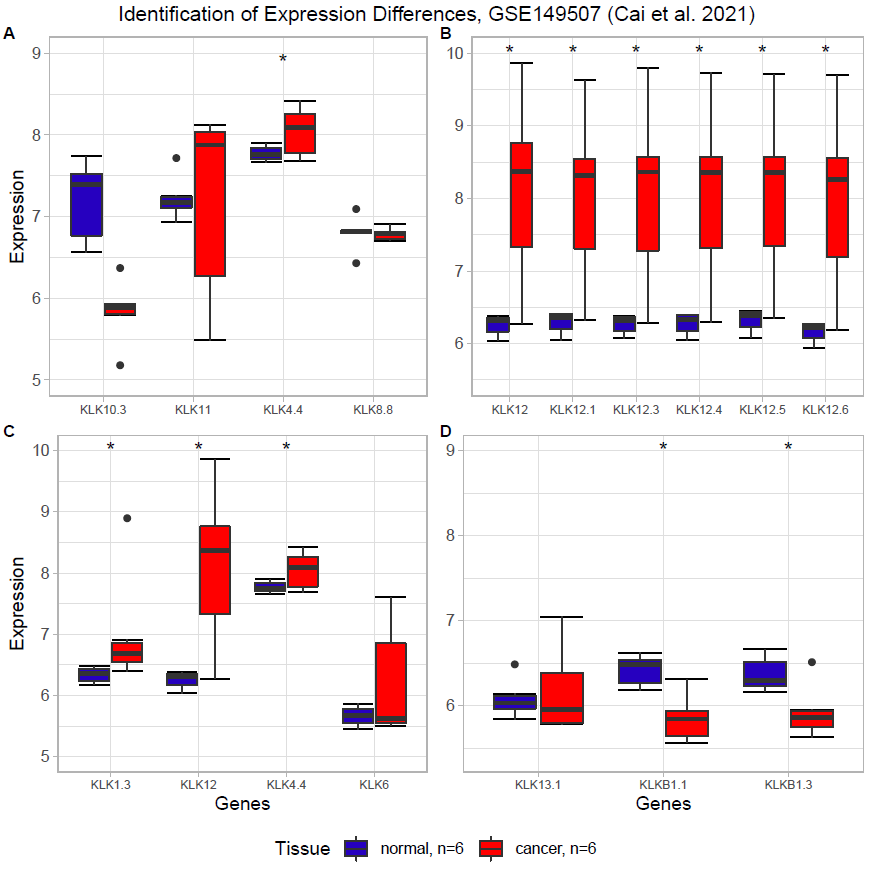
\includegraphics[width=0.5\linewidth]{images/Expr_diff_kmeans_PCA_lung} 

}

\end{figure}

\hypertarget{logistsic-regression}{%
\subsection{5. Logistsic regression}\label{logistsic-regression}}

Kallikrein mRNA or protein expression are already established in
clinical practice as biomarkers especially in prostate cancer (Diamandis
et al.~1998). Testing whether the identified genes with a significant
expression difference were likely to predict tissue type, logistic
regression was chosen. The basic assumptions for logistic regression
are: 1. Independence of errors, every observation has to be separate
from the others. 2. Linearity of the continuous variables in logit - the
relationship between the variable and their logit transformed outcome
should be linear. 3. Absence of multicollinearity or redundancy. 4. No
outliners with a strong influence. 5. For every independent variable
there should be at least ten outcomes (Stoltzfus 2011).

These assumptions reveal the shortcomings of the used data and explain
the experienced problems with logistic regression. First, the main
limitation of the used dataset is the low number of included microchips.
The number of microchips has also been further reduced by splitting the
data in a training dataset (eight microchips) and testing dataset (four
microchips). Therefore, expected problems of high standard errors and
large beta-coefficients for the independent variables were encountered
when including more then one independent variable. This phenomenon is
also called overfit-model. For most individual genes with a significant
expression difference the described problems were encountered. The only
exceptions were KLK4.4 and KLK12.

Second, although genes with a correlation equal to one were removed,
some genes are still highly correlating. This is primarily true for the
different isoforms of the same gene as visualized in figure x, plot B.
Therefore, the effect of collinearity would probably cause problems,
even if more microchips were included. Hence a second cleanup, removing
genes with high correlation (e.g.~corr \textgreater{} 0.8), would
probably be necessary. As mentioned above, KLK4.4 and KLK12 (and its
isoforms) were the only gene where the standard error of the independent
variable was not abnormaly high. In both cases the p-value was not
significant. In contrast, the prediction of these univariant models were
surprisingly accurate. The model with KLK4.4 could predict the tissue
type of three out of four microchips correctly, whereas the model with
KLK12 predicted every tissue type right. However, a closer look at the
probabilities reveals that these models are not reliable. The
probabilities for normal to be cancer tissue were mostly over a quarter,
indicating a high uncertainty.\\
In conclusion, the p-values of the independent variable in the models
were not significant, the standard errors were high and the predictions
probabilities were not accurate. These results were not surprising
considering the low sample size.

\begin{Shaded}
\begin{Highlighting}[]
\CommentTok{#Output of the two models !}
\end{Highlighting}
\end{Shaded}

\hypertarget{discussion}{%
\subsection{Discussion}\label{discussion}}

The aim of this project was to analyse whether the expression of
Kallikrein genes in given datasets show potential biomarker
characteristics and to compare the output of statistical analysis to
already existing literature, to verify the results. Principal component
analysis with breast cancer microarray data GSE65216 (Maire et al.~2013)
provides greater insight into the expression patterns within the
dataset. PCA shows that some samples are more dominated by KLK11 and
KLK11.2 expression. In addition, it shows that TNBC mutations are
influenced by the expression of KLK5 and KLK6. In the heatmap four genes
were identified, which were over-expressed in at least two of the five
mutation specific microchips. KLK10.3, KLK6 for Her2, KLK11, KLK11.2 for
LumA. Those four genes are also identified as one of the twelve main
loadings of the PCA. In a previous study (Haritos et al.~2018) KLK6
expression was found to be generally down-regulated in breast cancer
tissue, but in HER2 and TNBC positive tumors KLK6 was over-expressed.
Those findings are only reflected to a limited extend in this analysis.
Only Her2 was found to be significantly higher expressed than LumA. TNBC
was not significantly higher expressed compared to the other mutations.
Another study from Michaelidou et al.~reported a higher expression of
KLK8 in TNBC and Her2 positive tumors compared to LumA and LumB positive
tumors. However, this analysis could only confirm significant TNBC
over-expression for the isoform KLK8.5 compared to LumA and LumB.
Nevertheless, the boxplots of KLK8.4 and KLK8.5 show the trend of Her2
and TNBC over-expression. KLK11 shows the highest expression in breast
cancer in the research of Sano et al., 2007 , thus it confirms the
result of PCA that KLK11 is up-regulated. In summary, the conducted
analysis could partially conform the findings from other research
groups. The differences can probably be explained by the small amount of
samples used in this analysis. In conclusion Kallikrein gene expression
can be used for identifying tumor subtypes and even predict the outcome
for a patient (Haritos et al.~2018). Analysis of the lung cancer
microarray GSE149507 (Cai et al.~2021) demonstrated differences in the
expression of some KLKs between the cancerous and normal tissues. The
result showed that KLK4.4 was significantly higher expressed in cancer
tissue. While in normal tissue KLK10.3 expressed significantly higher.
The finding of decreased KLK11 expression in lung cancer by Sasaki et
al.~could not be confirmed. Rather, the median of cancer tissue samples
is significantly higher. Also, the conspicuity of significant high
expression of KLK12 and its isoforms in cancer tissue was detected.
Documented over-expression of KLK12 could not be found in the
literature, but functional studies identified KLK12 as a pro-angiogenic
factor. In conclusion, characteristical biomarker expression has been
found and also verified by comparison with literature. High overlap of
our results with literature confirms the right usage of methods, and
also indicate that results who couldn't be verified by literature
comparison, like expression values for KLK12, could be potentially
interesting to investigate.

\newpage

\hypertarget{references}{%
\subsection{References}\label{references}}

Ardlie, K.G., Deluca, D.S., Segre, A.V., Sullivan, T.J., Young, T.R.,
Gelfand, E.T., Trowbridge, C.A., Maller, J.B., Tukiainen, T., Lek, M.,
et al.~(2015). The Genotype-Tissue Expression (GTEx) pilot analysis:
Multitissue gene regulation in humans. Science 348, 648-660.\\
Borgoño, C.A., and Diamandis, E.P. (2004). The emerging roles of human
tissue kallikreins in cancer. Nature Reviews Cancer 4, 876-890.\\
Cai, L., Liu, H., Huang, F., Fujimoto, J., Girard, L., Chen, J., Li, Y.,
Zhang, Y.-A., Deb, D., Stastny, V., et al.~(2021). Cell-autonomous
immune gene expression is repressed in pulmonary neuroendocrine cells
and small cell lung cancer. Communications Biology 4.\\
Diamandis, E.P. (1998). Prostate-specific Antigen: Its Usefulness in
Clinical Medicine. Trends in Endocrinology \& Metabolism 9, 310-316.\\
Dinkelacker, M. (2007). A database of genes that are expressed in a
tissue-restricted manner to analyse promiscous gene expression in
medullary thymic epithelial cells. Diplomarbeit
(Albert-Ludwigs-Universitaet).\\
Dinkelacker, M. (2019). Chromosomal clustering of tissue restricted
antigens. Dissertation (University Heidelberg). Dubey, A.K., Gupta, U.,
and Jain, S. (2016). Analysis of k-means clustering approach on the
breast cancer Wisconsin dataset. International Journal of Computer
Assisted Radiology and Surgery 11, 2033-2047.\\
Fischer, J., and Meyer-Hoffert, U. (2013). Regulation of
kallikrein-related peptidases in the skin -- from physiology to diseases
to therapeutic options. Thromb Haemost 110, 442-449.\\
Haritos, C., Michaelidou, K., Mavridis, K., Missitzis, I., Ardavanis,
A., Griniatsos, J., and Scorilas, A. (2018). Kallikrein-related
peptidase 6 (KLK6) expression differentiates tumor subtypes and predicts
clinical outcome in breast cancer patients. Clinical and Experimental
Medicine 18, 203-213.\\
Kont, V., Laan, M., Kisand, K., Merits, A., Scott, H.S., and Peterson,
P. (2008). Modulation of Aire regulates the expression of
tissue-restricted antigens. Molecular Immunology 45, 25-33.\\
Lattin JE, S.K., Su AI, Walker JR, Zhang J, Wiltshire T, Saijo K, Glass
CK, Hume DA, Kellie S, Sweet MJ (2008). Expression analysis of G
Protein-Coupled Receptors in mouse macrophages. Immunome Res. 4:5.\\
Lenga Ma Bonda, W., Iochmann, S., Magnen, M., Courty, Y., and Reverdiau,
P. (2018). Kallikrein-related peptidases in lung diseases. Biol Chem
399, 959-971.\\
Lonsdale, J., Thomas, J., Salvatore, M., Phillips, R., Lo, E., Shad, S.,
Hasz, R., Walters, G., Garcia, F., Young, N., et al.~(2013). The
Genotype-Tissue Expression (GTEx) project. Nature Genetics 45,
580-585.\\
Maire, V., Némati, F., Richardson, M., Vincent-Salomon, A., Tesson, B.,
Rigaill, G., Gravier, E., Marty-Prouvost, B., De Koning, L., Lang, G.,
et al.~(2013). Polo-like Kinase 1: A Potential Therapeutic Option in
Combination with Conventional Chemotherapy for the Management of
Patients with Triple-Negative Breast Cancer. Cancer Research 73,
813-823.\\
Michaelidou, K., Ardavanis, A., and Scorilas, A. (2015). Clinical
relevance of the deregulated kallikrein-related peptidase 8 mRNA
expression in breast cancer: a novel independent indicator of
disease-free survival. Breast Cancer Research and Treatment 152,
323-336.\\
Roth, R.B., Hevezi, P., Lee, J., Willhite, D., Lechner, S.M., Foster,
A.C., and Zlotnik, A. (2006). Gene expression analyses reveal molecular
relationships among 20 regions of the human CNS. Neurogenetics 7,
67-80.\\
Sano, A., Sangai, T., Maeda, H., Nakamura, M., Hasebe, T., and Ochiai,
A. (2007). Kallikrein 11 expressed in human breast cancer cells releases
insulin-like growth factor through degradation of IGFBP-3. Int J Oncol
30, 1493-1498.\\
Sasaki, H., Kawano, O., Endo, K., Suzuki, E., Haneda, H., Yukiue, H.,
Kobayashi, Y., Yano, M., and Fujii, Y. (2006). Decreased Kallikrein 11
Messenger RNA Expression in Lung Cancer. Clinical Lung Cancer 8,
45-48.\\
Schmitt, M., Magdolen, V., Yang, F., Kiechle, M., Bayani, J., Yousef,
G.M., Scorilas, A., Diamandis, E.P., and Dorn, J. (2013). Emerging
clinical importance of the cancer biomarkers kallikrein-related
peptidases (KLK) in female and male reproductive organ malignancies.
Radiology and Oncology 47, 319-329.\\
Su, A.I., Cooke, M.P., Ching, K.A., Hakak, Y., Walker, J.R., Wiltshire,
T., Orth, A.P., Vega, R.G., Sapinoso, L.M., Moqrich, A., et al.~(2002).
Large-scale analysis of the human and mouse transcriptomes. Proceedings
of the National Academy of Sciences 99, 4465-4470.\\
Su, A.I., Wiltshire, T., Batalov, S., Lapp, H., Ching, K.A., Block, D.,
Zhang, J., Soden, R., Hayakawa, M., Kreiman, G., et al.~(2004). A gene
atlas of the mouse and human protein-encoding transcriptomes.
Proceedings of the National Academy of Sciences 101, 6062-6067.\\
Tailor, P.D., Kodeboyina, S.K., Bai, S., Patel, N., Sharma, S., Ratnani,
A., Copland, J.A., She, J.-X., and Sharma, A. (2018). Diagnostic and
prognostic biomarker potential of kallikrein family genes in different
cancer types. Oncotarget 9, 17876-17888. 10.18632/oncotarget.24947.\\
Uhlen, M., Fagerberg, L., Hallstrom, B.M., Lindskog, C., Oksvold, P.,
Mardinoglu, A., Sivertsson, A., Kampf, C., Sjostedt, E., Asplund, A., et
al.~(2015). Tissue-based map of the human proteome. Science 347,
1260419-1260419.\\
Yousef, G.M., Chang, A., Scorilas, A., and Diamandis, E.P. (2000).
Genomic Organization of the Human Kallikrein Gene Family on Chromosome
19q13.3--q13.4. Biochemical and Biophysical Research Communications 276,
125-133.\\
Yousef, G.M., Magklara, A., and Diamandis, E.P. (2000). KLK12 Is a Novel
Serine Protease and a New Member of the Human Kallikrein Gene
Family---Differential Expression in Breast Cancer. Genomics 69,
331-341.\\
Yousef, G.M., Yacoub, G.M., Polymeris, M.E., Popalis, C., Soosaipillai,
A., and Diamandis, E.P. (2004). Kallikrein gene downregulation in breast
cancer. British Journal of Cancer 90, 167-172.\\
Zhang, Y., Bhat, I., Zeng, M., Jayal, G., Wazer, D.E., Band, H., and
Band, V. (2006). Human kallikrein 10, a predictive marker for breast
cancer. 387, 715-721.

\end{document}
